% chapter3.tex -- en (English)
\chapter{Modification of \Bezeichnung}
This chapter describes how to ``mod'' this project:
\begin{compactitem}
	\item The hardware section primarily describes the installation of the additional circuit board containing the TinkerKit pushbuttons.
	\item The software part assumes a successful installation of the Arduino IDE on the working computer and further the knowledge of flashing an Arduino board using the IDE.
\end{compactitem}
%The hardware section primarily describes the installation of the
%additional circuit board containing the TinkerKit pushbuttons.\\
%The software part assumes an successful installation of the Arduino IDE
%on the working computer and also the knowledge of flashing an Arduino
%board using the IDE.

\section{Description of the additional TinkerKit Pushbuttons Board}
\label{sect:TinkerKitBoard}
Modern gaming controllers usually provide more switches than the
four cursor pushbuttons. There are often so-called shoulder buttons
in front of the controller's housing which are pressed by
the forefingers.

The {\Bezeichnung} enables the four TinkerKit connectors to add more
pushbuttons. Since the white TinkerKit connectors are wired to input
pins of the \textit{ATmega32U4} microcontroller, which provide a 10bit
A/D converter facility, several pushbuttons can act
\textbf{simultaneously} on each white TinkerKit connector. They are
distinguished by suitable voltage dividers:\\
On the prototype of the additional board each analogue TinkerKit
connector (white) provides two pushbuttons using the voltage dividers
33k : 22k resp. 33k : 47k. This results in the following voltages and
A/D values:

\begin{table}[h]
\centering
\renewcommand{\arraystretch}{1.5}
\begin{tabular}{p{0.20\textwidth}p{0.20\textwidth}p{0.20\textwidth}}
	\textbf{pushbutton}	&	\textbf{A/D value}	&	\textbf{voltage}\\
	no button			&	1023				&	5,00V\\
	47k button			&	601					&	2,94V\\
	22k button			&	410					&	2,00V\\
	both buttons		&	320					&	1,56V\\
\end{tabular}
\vspace{0.5cm}
\caption{A/D Values of the TinkerKit Pushbuttons}
\end{table}

The following pictures show the connection of the prototype board at the
\Bezeichnung. In the appendix there can be found a wiring conception and
the technical drawings of a printed circuit board which provides up to
three pushbuttons on each white TinkerKit connector.
 
\begin{figure}[!h]
\centering
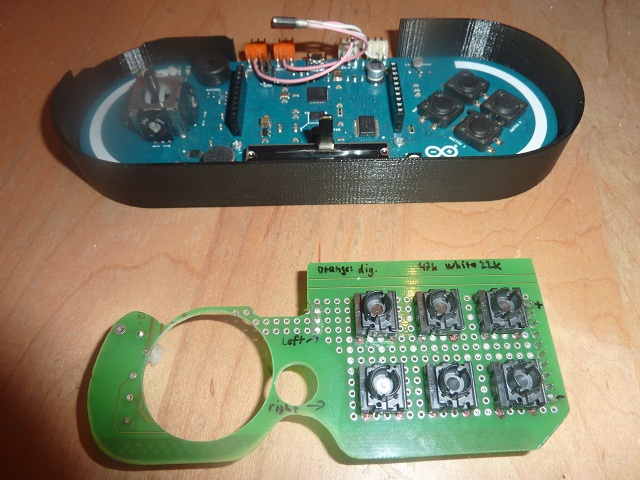
\includegraphics[width=0.85\textwidth]{esplora01.jpg}
\caption{Arduino Esplora and Additional TinkerKit Board (Prototype)}
\label{fig:esplora01}
\end{figure}

\begin{figure}[!h]
\centering
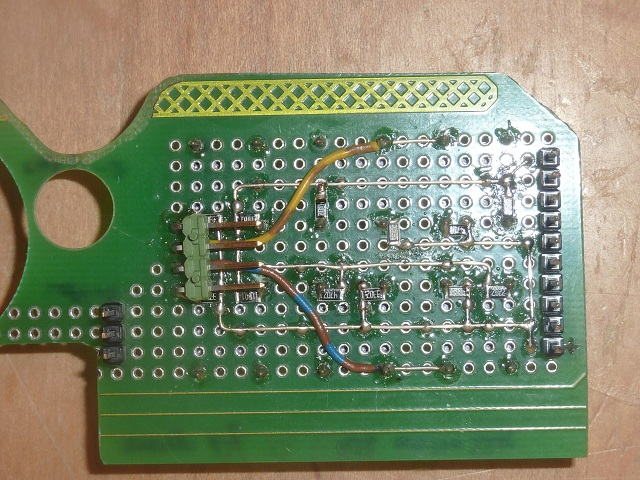
\includegraphics[width=0.85\textwidth]{esplora02.jpg}
\caption{Resistors of the Additional TinkerKit Board}
\label{fig:esplora02}
\end{figure}

\newpage
\begin{figure}[!h]
\centering
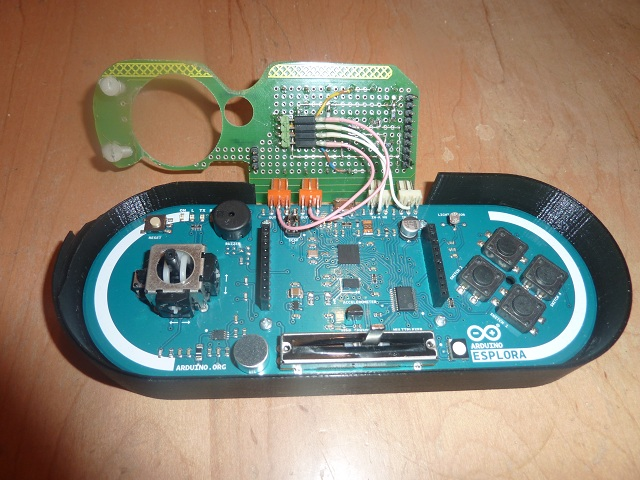
\includegraphics[width=0.85\textwidth]{esplora03.jpg}
\caption{Connection of the TinkerKit Board at the Arduino Esplora}
\label{fig:esplora03}
\end{figure}

\begin{figure}[!h]
\centering
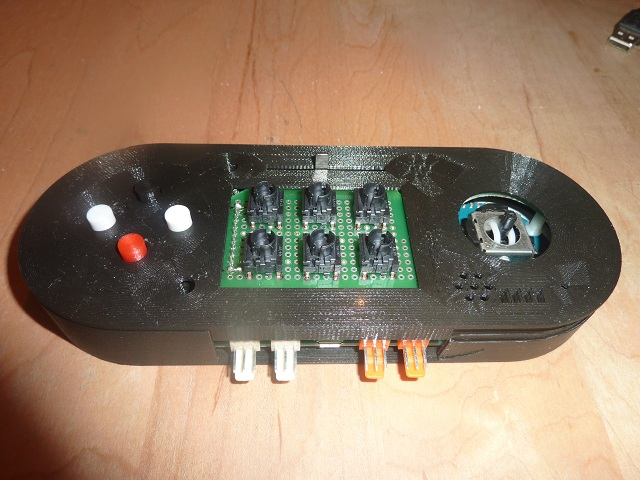
\includegraphics[width=0.85\textwidth]{esplora04.jpg}
\caption{Additional TinkerKit Board Inside the Housing}
\label{fig:esplora04}
\end{figure}



\newpage
\section{Description of the Arduino Sketch for \Bezeichnung}
\subsection{Installation of the Arduino-IDE}
A complete description of how to use the \textit{Arduino Web Editor} or
the \textit{Arduino Desktop IDE} can be found at
\url{https://www.arduino.cc/en/Guide/HomePage}. Each user should decide
the preferred variant individually.

\subsection{Code Adjustments}
An Arduino Edsplora Board flashed with the downloaded sketch
\texttt{EsploraGamingController.ino} emulates a USB mouse and a USB
keyboard as described in chapter \ref{cha:manual}.

The easiest way to adjust the code is to change the values of the
two-dimensional array variable \texttt{gl\_modeKeycodes} according to
the own preferences and to re-flash the Arduino Esplora board. A list of
non-ASCII characters can be found in the file
\texttt{Esplora\_ExtendedKeycodes.txt}.\\
The value 0 activates a \textbf{mouse action} which is implemented
in code for the actuator:
\begin{table}[h]
\centering
\renewcommand{\arraystretch}{1.5}
\begin{tabular}{|p{0.25\textwidth}|p{0.70\textwidth}|}
\hline
\textbf{actuator}		&	\textbf{mouse action on value 0}\\
\hline
	joystick movement	&	mouse movement\\
\hline
	joystick pressure	&	left click\\
\hline
	TinkerKit orange	&	left/right click\\
\hline
	TinkerKit white		&	\textbf{no mouse function!}\\
\hline
	slider				&	scrolling wheel\\
\hline
	light sensor		&	right click\\
\hline
	cursor pushbuttons	&	\textbf{no mouse function!}\\
\hline
\end{tabular}
\vspace{0.5cm}
\caption{Default Mouse Actions of All Actuators}
\end{table}

The value 255 (or the constant \texttt{FUNCT\_DISABLED}) disables an
actuator completely.

All analogue acutators supply a value between 0 and 1023, since they are
taken by a 10-bit A/D converter. The joystick 10-bit values determine
the speed of the mouse movement. When keyboard codes are assigned to the
joystick the repetition rate of the corresponding key is also given by 
joystick displacement.\\
The slider emulates the rotation of the mouse scroll wheel. Here the
displacement determines the speed of the scroll commands. To to stop the
scrolling, the slider has to be moved slightly back towards the middle
position. This works even when the slider position value itself would
cause scrolling. The slight push back causes the stop of scrolling.\\
At the white TinkerKit connectors the A/D converter is used to detect
a combination of two pushbuttons on each connector. The additional
TinkerKit board contains a suitable combination of voltage divider
resistors. The limits are defined in the array variable
\texttt{TINKERKIT\_LEVEL}. When adjusting these limit you have to take
care that they are in the middle between the measured values to ensure
a proper detection.\\
The light sensor gives a 10-bit value too, but it's difficult to use it
as an actuator. Even small changes in the lighting conditions caused by
accidental covering of the sensor lead to erroneous actions. Therefore
it isn't recommended to use the light sensor as an actuator. You should
disable it.


\subsection{Structure of the Code}
This section explains the most important \texttt{\#define}s, variables
and functions of the source code:

\subsubsection*{serial interface (UART)}
In addition to the emulation of mouse and keyboard this sketch provides
a virtual serial port (UART) using a baud rate of 9600. In Windows this
serial port is shown in the device manager as a COM port and in
GNU/Linux there is a device file \texttt{/dev/ttyACM<x>}. \todo{clean up
the UART output}The data transmitted via this serial port aren't
properly structured yet!

\subsubsection*{\texttt{\#define}}
\uline{\texttt{\#define SERIAL\_DEBUG}}\\
Enables/disables debug messages at the serial interface (UART)

\uline{\texttt{\#define LOOP\_DELAY}}\\
Defines a delay in milli seconds between two cycles of the main loop.
The smaller this value is the faster the Arduino Esplora Board reacts on
changes at the actuators. Especially the mouse cursor speed due to
joystick movements depends on this timing value.\\
Too short delay values might not work properly because of bouncing
bushbuttons. This will result in double actions if the button is pressed
only once!

\subsubsection*{Variables}
\uline{variable \texttt{byte gl\_mode}}\\
Holds the currently selected assignment mode as a value from 0 to 7.

\uline{array variable \texttt{char* gl\_modeNames[8]}}\\
Contains the names of the eight assignment modes. When selecting a mode
its name (denomination) will be transmitted via the serial interface
(UART).

\uline{two-dimensional array variable \texttt{char gl\_modeKeycodes[8][18]}}\\
Stores byte values of the keyboard and mouse commands for all
actuators:\\
\begin{tabular}{ll}
0		&	mouse command\\
1-254	&	key code\\
255		&	disabled\\
\end{tabular}

\subsubsection*{Functions}
\uline{function \texttt{void setup()}}\\
This is a default function of any Arduino sketch. It is called once when
the arduino board starts and it is used here to initialize the variable
values and for calibration of analogue sensors, especially of the
joystick displacement.

\uline{function \texttt{void loop()}}\\
This is a default function of any Arduino sketch. After \texttt{setup()}
it is called in an endless loop. Here the actuator values are polled.

\uline{function \texttt{void setMode(byte mode)}}\\
Establishes the given assignment mode (0 to 7):
\begin{compactitem}
	\item sets the variable \texttt{gl\_mode} to the given value
	\item Sets the colour of the three-colour LED
	\item Sends the name of the selected assignment mode via UART
\end{compactitem}

\uline{function \texttt{unsigned int readTinkerkitInput(byte whichInput)}}\\
Reads the TinkerKit input connectors using the function
\texttt{readChannel(byte channel)}.

\uline{function \texttt{unsigned int readChannel(byte channel)}}\\
This function supersedes the identically named function of the
Arduino library \texttt{Esplora}. The hardware selection of the
TinkerKit connector is done by a multiplexer chip on the Arduino Esplora
Board.

\uline{function \texttt{byte tinkerkitWhiteSwitches(unsigned int analogue)}}\\
Evaluates the pressed key combination on the white TinkerKit connectors.
It contains the local variable \texttt{const unsigned int 
TINKERKIT\_LEVEL[4]} where the analogue limits are defined to detect the
pressed TinkerKit pushbutton combination. These limits can be evaluated
by sending the values via UART when a button combination is pressed. The
measured values should be fairly in the middle between two limit
values defined in this variable. The other way to define the limits is 
to set them to the middle value between two consecutive button
combinations.\\
In order for this function to work properly, the voltage divider
resistors must have been dimensioned suitably and correctly!


\section{Prospect on Planned Developments}
\begin{enumerate}
\item The user can change the assignments directly on the device without
      changing the source code 
\item Storage of changed assignments in the EEPROM of the
      \textit{ATmega32U4}
\item Definition of several keystrokes on one actuator
\item Definition of values for mouse actions (1\dots31?)
\item Clean up of the outputs at the serial interface
\end{enumerate}
